\chapter{Arbejdsproces}

\section{Udviklingsmodeller (JS, PO)}
Med udgangspunkt i ISE-undervisningen\footnote{Indledende System Engineering - ASE, fag på 2. semester} er projektarbejde opbygget omkring ASE-modellen som ses på figur \ref{fig:ASE_model}. ASE-modellen er opbygget i 2 faser. En fællesfase og en fag specifik fase. 


\begin{figure}[htbp]
  \centering
    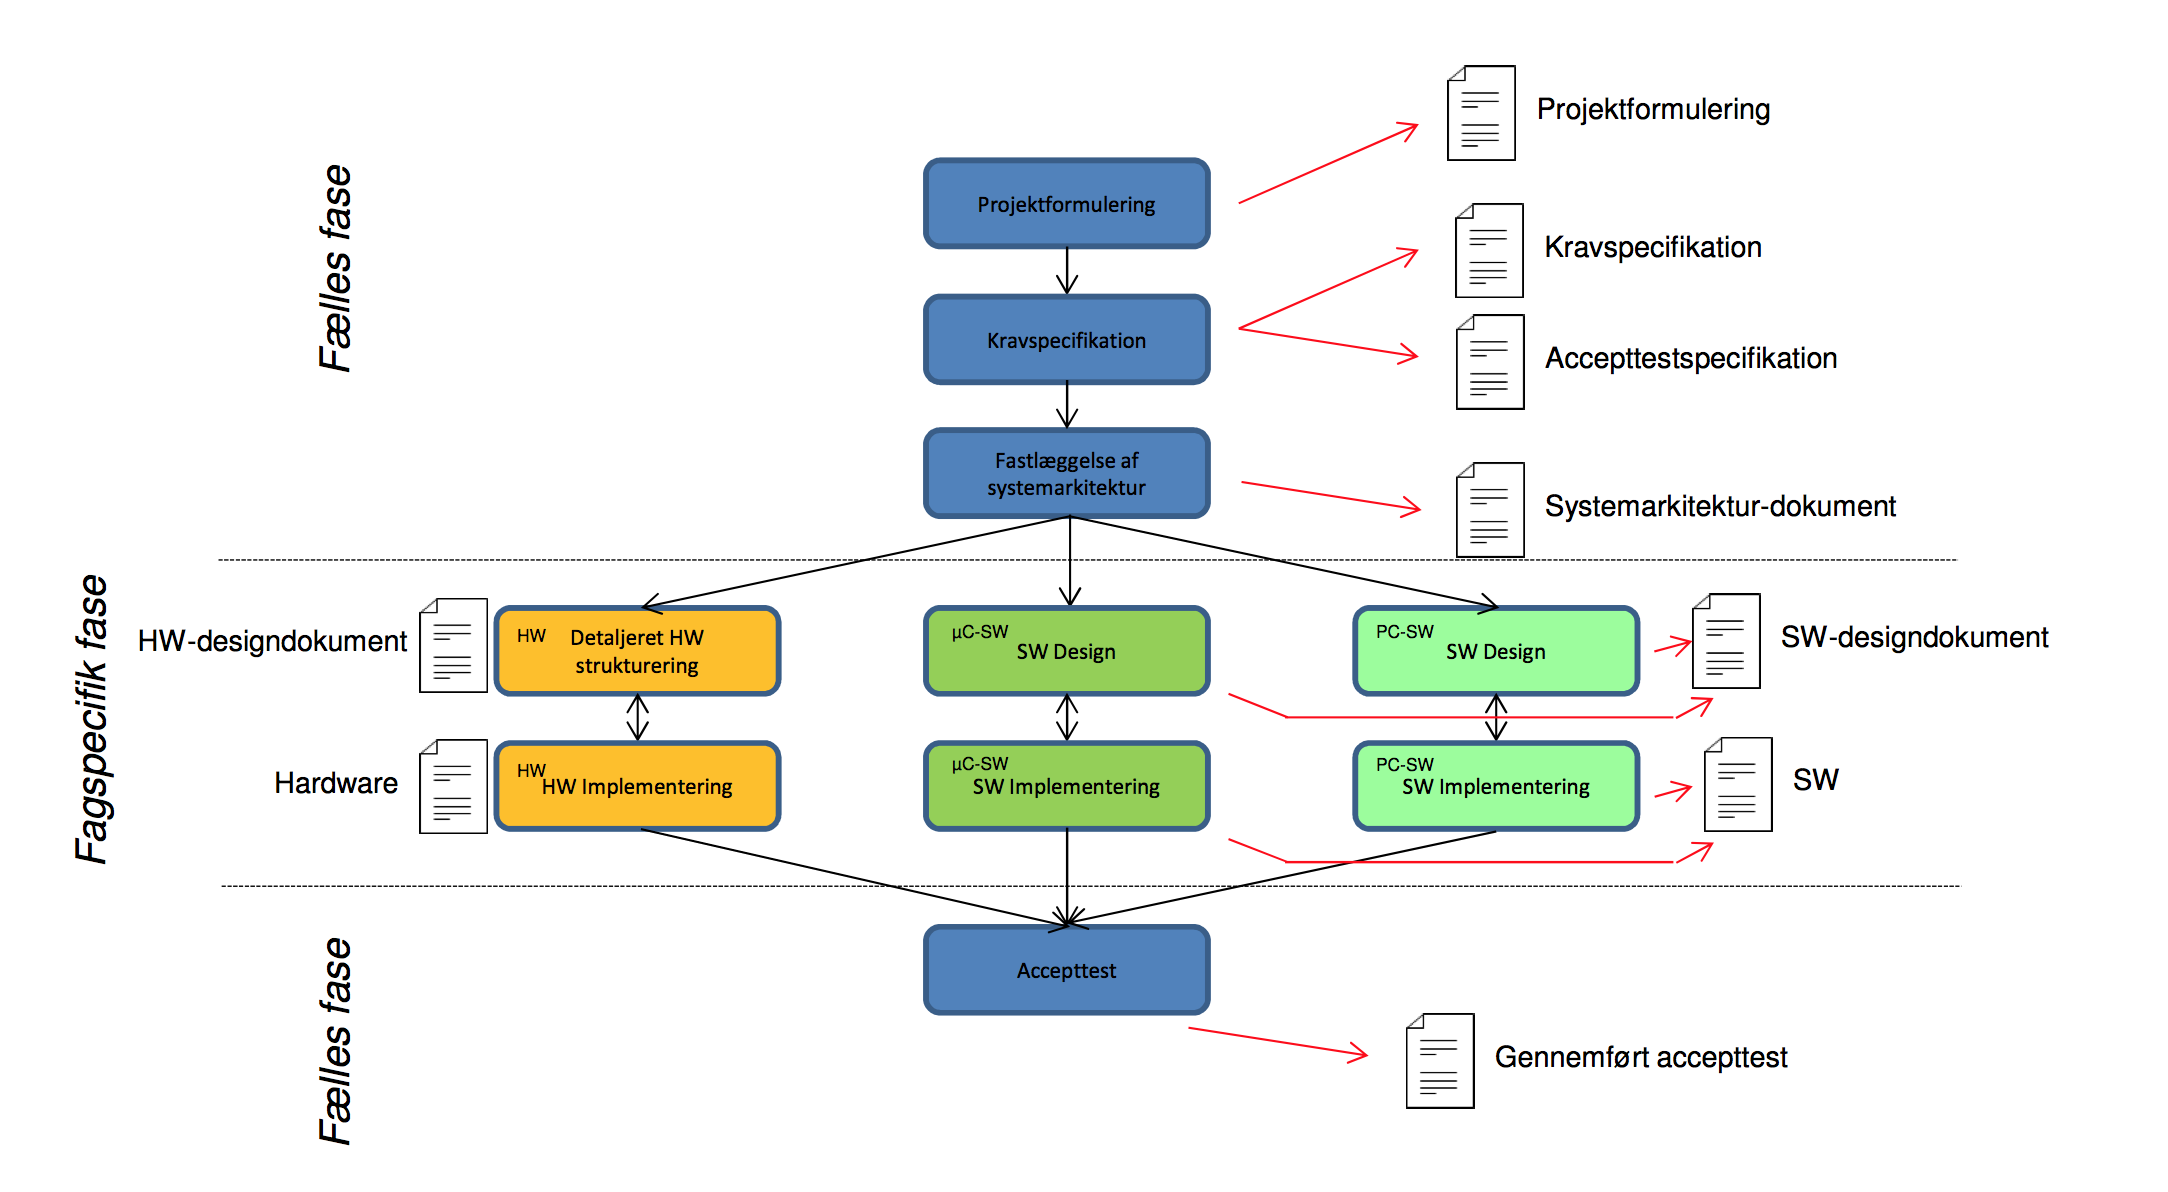
\includegraphics[width=0.8\textwidth]{billeder/ASE-modellen}
    \caption{ASE-modellen}
    \label{fig:ASE_model}
\end{figure}

I fællesfasen arbejde hele gruppen sammen omkring udarbejdelse af de forskellige deldokumenter. 
I den fag specifikke fase deles gruppen op i mindre teams for at udvikle de fag specifikke deldokumenter. 

ASE-modellen tager udgangspunkt i V-modellen som ses på figur \ref{fig:V_model}.   

\begin{figure}[htbp]
  \centering
    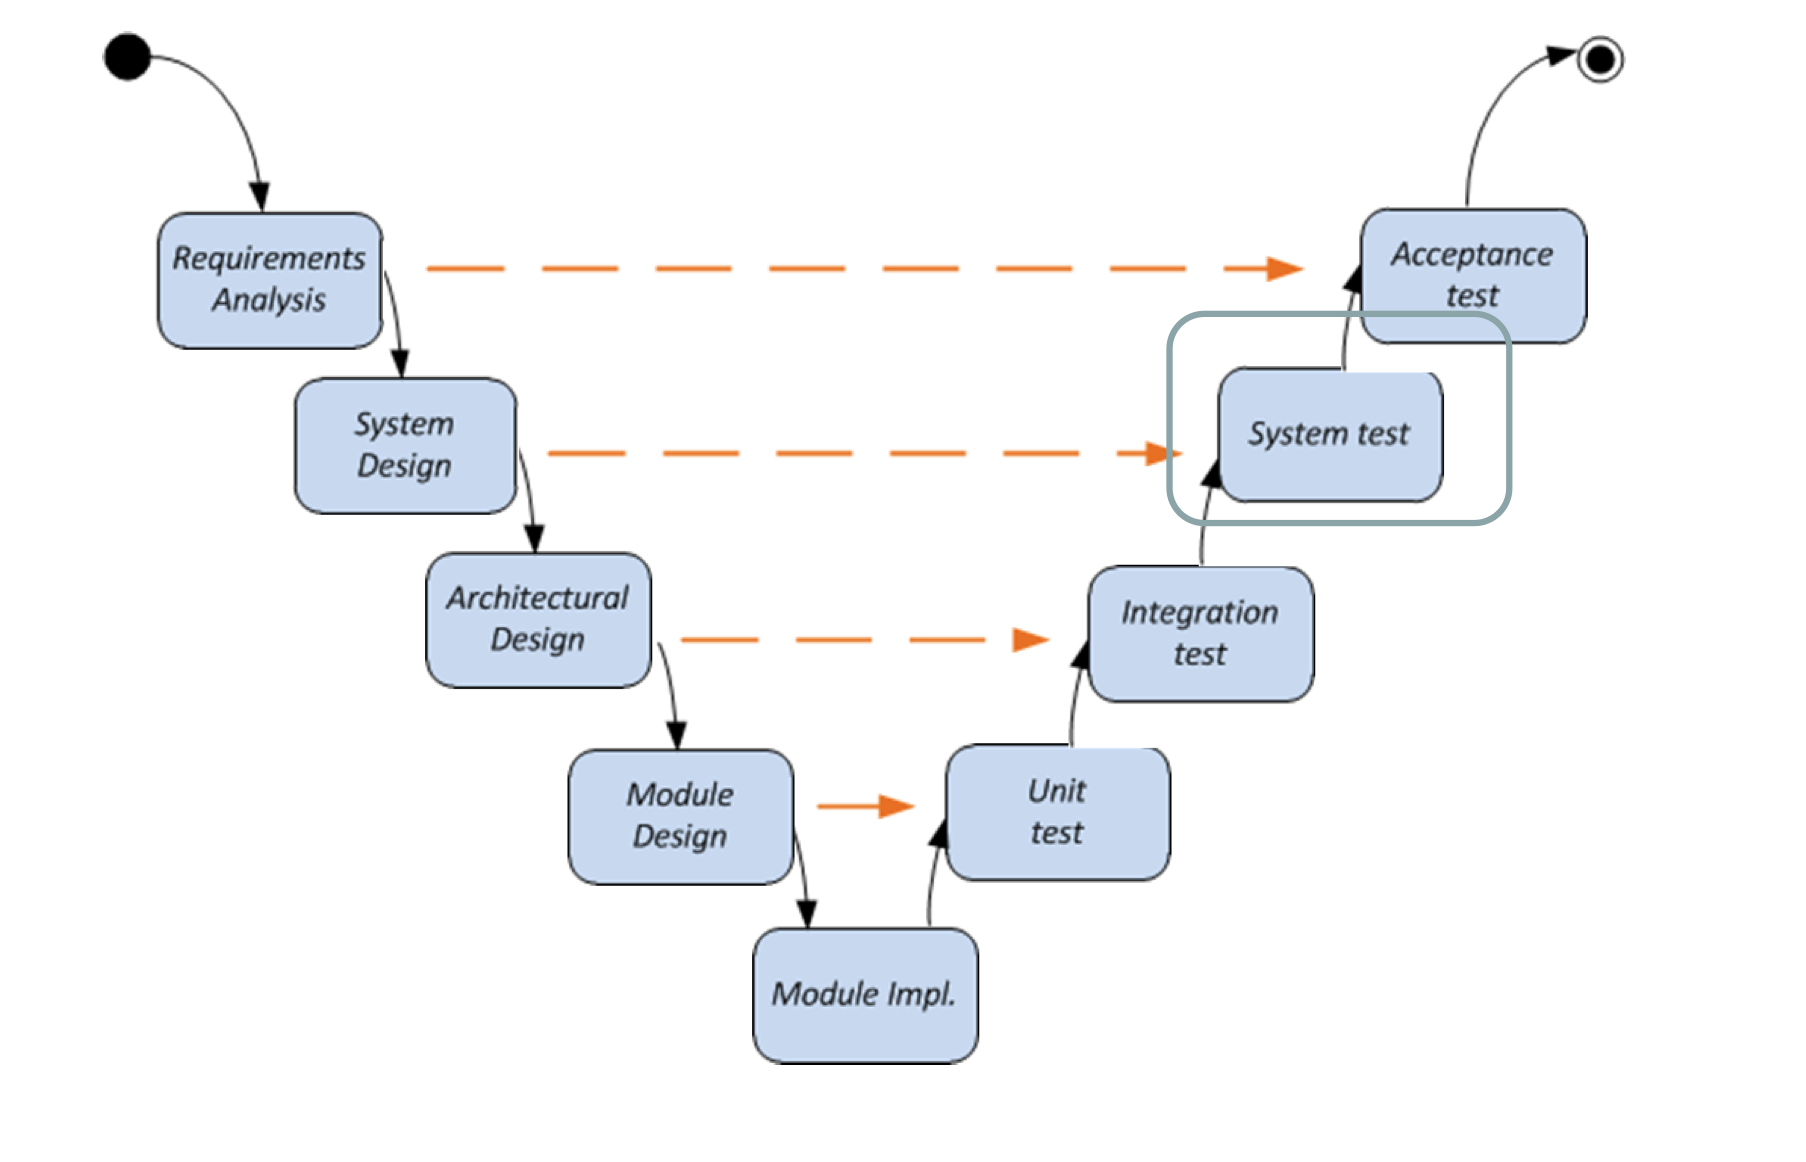
\includegraphics[width=0.8\textwidth]{billeder/V-modellen}
    \caption{V-modellen}
    \label{fig:V_model}
\end{figure}

V-modellen ses på figur \ref{fig:V_model}. Ved at benytte V-modellens opbygning færdiggøres en fase inden en ny påbegyndes. Og ydermere planlægges testen af alle faserne parallelt med at fasen udarbejdes. F.eks udarbejdes accepttesten samtidigt med at kravespecifikationen udarbejdes.  

\section{Møder, tidsplan, logbog og referater (PO)}

I forbindelse med projektforløbet er der afholdt en række møder. Vejledermøder, gruppemøder samt reviewmøder.

Vejledermøder er forbindelsen mellem gruppen og gruppens vejleder. Her har det været muligt at få løbende feedback samt et indblik i om det der forventes også er det gruppen forventer. Vejledermøder har været fastlagt til én i ugen. Det er næsten opretholdt, dog med enkelte aflysninger.

Gruppen har hver uge holdt mindst et, nogle gange flere møder. Disse møder er brugt til at afklare uoverensstemmelser og planlægning af den kommende uge. Under gruppemøderne er der 2 gange brugt tid på en trivsels runde. Her har det været muligt at give ris/ros til gruppen og eller enkelte. Gruppemøderne startede lidt løst, men dette blev hurtigt ændret til at have en fast mødeholder, som styrede mødets gang. Tidsplanen er under gruppemøderne blevet revideret, således at den altid var opdateret til vejledermøderne. Gruppen har fra start udarbejdet en gruppekontrakt\footnote{Gruppekontrakten findes på bilags cd under navnet: Gruppekontrakt.pdf}. Gruppekontrakten har dannet grundlag for forventningerne til gruppen og dens medlemmer.

Reviewmøder har fungere således at gruppen enten udførte review på en anden gruppen og herefter fremlagde dette. Omvendt modtog gruppen lignende review fra andre grupper. Disse review førte ofte til uklarheder, som gruppen herefter måtte tage stilling til i gruppemødet.

Alle møder blev ajour ført med logbog og mødereferat. Her har gruppen haft en fast sekretær. 

\section{HW/SW teams}

\subsection{Hardware teamet (PO)}
Hardware teamet bestående af: Jakob, Mick, Poul og Simon har arbejdet meget sammen om opgaven. Samarbejde er nøgleordet for dette team. Alle fire har hovedsagligt deltaget i alle opgaver herunder.  

\subsection{Software teamet (BS)}
I software gruppen bestående af Bjørn, Jeppe og Jesper har vi arbejdet sammen under de indledende faser og først i den detaljerede designfase har vi delt opgaverne op.
Der fra har vi arbejdet individuelt, men dog med regelmæssige møder og afklaring for at sikre at interface aftaler og lignende stadig blev overholdt.


\section{Arbejdsfordeling}
 
Kapitler og afsnit er angivet med forfatter, hvor gruppen ikke har været fællesforfatter. Oftest har der været flere om emnet, men kun én eller to forfattere. Derfor beskrives der herunder hvem der har haft hvilke arbejdsområder.  

Arbejdsfordelingen er herunder beskrevet. 

\subsection{Hardware} 
Hele hardware teamet har deltaget på lige fod i den foranliggende process mht. til arkitektur og design. Herefter har enkelte været forfattere på dele af hhv. rapport og dokumentation. Heraf ses at Jakob og Simon har stået for en del af indskrivningen, mens Mick og Poul har stået for implementeringen og den tilhørende test.
Vi har som team været samlet omkring fejlfinding af de enkelte moduler.  

\subsection{Software}


\subsection{Andet}

Opsætning af \LaTeX, både dokumentation og rapport
Hovedansvarlige: Mick, Poul 

Sekretærarbejde - Bestående af Logbog samt mødereferater
Hovedansvarlig: Simon

Mødeleder - Afholdelse af møder, status, samt tavlestyring 
Hovedansvarlig: Poul




